\section{Unified Theoretical Framework for Optimizers}
\label{sec:unified-theoretical-framework}

\subsection{Universal Meta-Pipeline}
\label{sec:meta-pipeline}

\subsubsection{Operational Steps}
\label{sec:meta-pipeline-steps}

Modern LLM optimizers are usually named after their most visible local
mechanism: an adaptive moment estimator, a matrix preconditioner, a low-rank
projection, a sign map, a compressed state, or a sharpness-aware correction.
Such descriptions are useful for implementation, but they make cross-method
comparison difficult because they do not say \emph{where} the mechanism enters
the update.  We therefore introduce a \emph{Universal Meta-Pipeline}: a
process-level abstraction that aligns the optimizers considered in this survey
to a common single-step update template.  Its purpose is to expose the
operation site of each method, to
separate primary mechanisms from defaults, and to prepare the bridge to the
LMO-driven geometric view in Section~\ref{sec:lmo-four-axis}.

\paragraph{Formal setup.}
Let $W_t\in\mathbb{R}^{m\times n}$ be a two-dimensional parameter tensor,
$G_t\in\mathbb{R}^{m\times n}$ its training signal, and
$\mathcal{S}_{t-1}$ the optimizer state before the update.  Five internal
operators $\mathbf{S1}$--$\mathbf{S5}$, each of which may degenerate to the
identity, transform $G_t$ into a signed parameter increment $\Delta_t$:
\begin{equation}
  \Delta_t =
  \mathbf{S5}\!\left(
    \mathbf{S4}\!\left(
      \mathbf{S3}\!\left(
        \mathbf{S2}\!\left(\mathbf{S1}(G_t)\right);\,\mathcal{S}_{t-1}
      \right);\,\mathcal{S}_{t-1}
    \right);\,\mathcal{S}_{t-1},\,W_t
  \right),\quad
  W_{t+1}=W_t+\Delta_t .
  \label{eq:meta_pipeline}
\end{equation}
The internal state $\mathcal{S}_t$ is updated within $\mathbf{S3}$ and is made
available to all downstream stages.  One-dimensional parameters (biases,
normalization coefficients, and other vector-like tensors) follow the same
pipeline, with matrix operations at $\mathbf{S2}$ and $\mathbf{S4}$ contracting
to element-wise equivalents or identity maps.  Figure~\ref{fig:meta_pipeline}
illustrates the pipeline for one training step.

\begin{figure}[t]
  \centering
  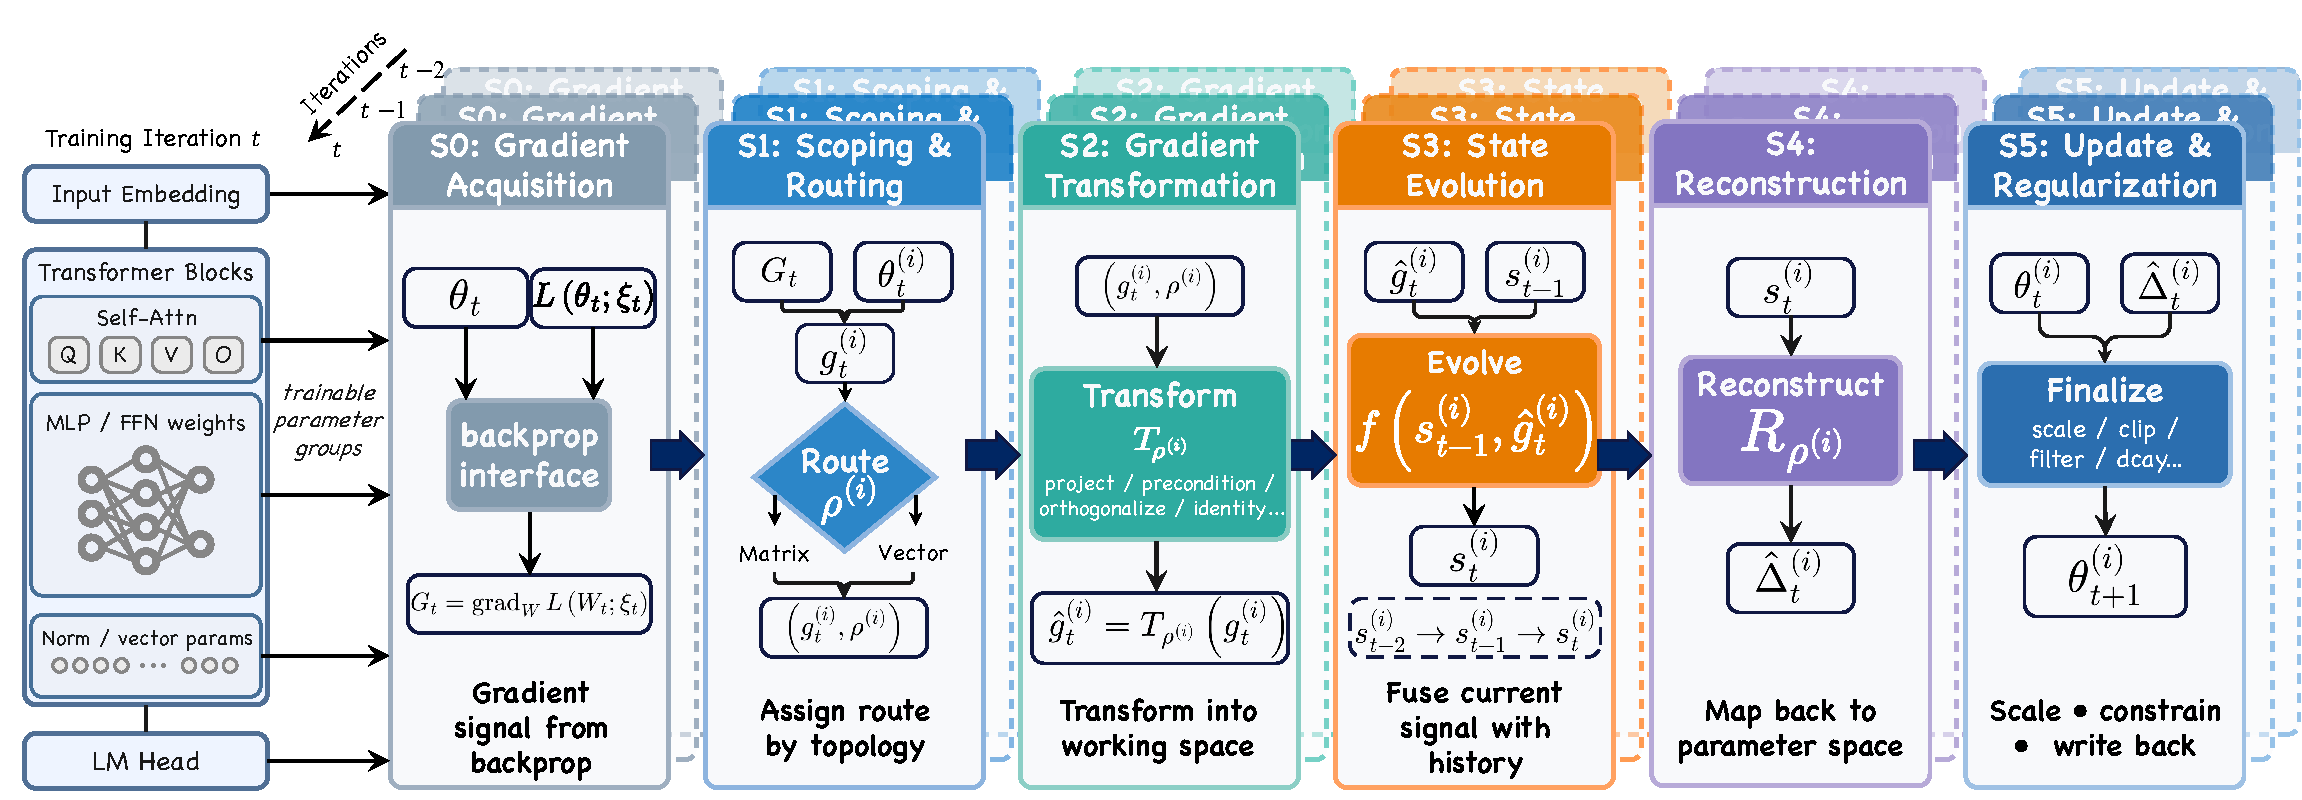
\includegraphics[width=1.0\linewidth]{figures/meta_pipeline.pdf}
  \caption{Universal meta-pipeline for one optimizer step.  The training system
  provides a gradient or higher-order signal (S0), which the optimizer
  processes through five internal stages for each parameter group.}
  \label{fig:meta_pipeline}
\end{figure}

\paragraph{S0: Training Signal Acquisition.}
Before the internal optimizer stages begin, the training system supplies a
signal.  We write this interface as S0 because it determines what information
the update pipeline is allowed to use.  The standard case is
\emph{first-order backpropagation} (FO),
$G_t=\nabla_W\mathcal{L}(W_t;\xi_t)$.  Some optimizers replace $G_t$ with a
\emph{variance-reduced} estimator, for example a STORM-style correction
$\tilde{G}_t=G_t-G_{t-1}^{\xi_t}+M_{t-1}$.  Others add
\emph{curvature-augmented} signals through Hessian-vector products or
Hutchinson diagonal estimates,
$h_t\approx u\odot (Hu)$ with $u\sim\mathcal{N}(0,I)$, as in
Sophia~\cite{liu2023sophia}.  Zeroth-order methods are treated as a boundary
case in this paper: their main contribution is often signal acquisition from
function values rather than the downstream update transformation, so they are
not part of the main T1--T5 update-mechanism taxonomy.

\paragraph{S1: Parameter Scoping and Routing.}
The first internal stage partitions the full parameter set
$\{\theta^{(i)}_{t-1}\}$ and assigns a routing label $\rho^{(i)}$ to each
group based on tensor topology and module type:
\begin{equation}
  \rho^{(i)} = \mathcal{R}\!\bigl(
    \mathrm{shape}(\theta^{(i)}),\;
    \mathrm{module\text{-}type}(\theta^{(i)})
  \bigr).
  \label{eq:routing}
\end{equation}
Equivalently, S1 outputs a partition
$\mathcal{P}=\{P_k\}_{k=1}^{K}$ together with the processing rule attached to
each group.  All downstream stages condition on $\rho^{(i)}$.  The common
partition separates two-dimensional matrices---which admit matrix-geometric
operations such as SVD decomposition, Kronecker factorization, and low-rank
projection---from vector-like parameters handled by element-wise rules.  Finer
partitions include attention-head blocks, per-layer groups, and
topology-dependent hybrid routes.  When all parameters share a single route,
S1 is an identity, as in standard AdamW.  When routing is nontrivial, the same
optimizer may apply different downstream operators to matrix, vector, or
module-specific parameter groups.

\paragraph{S2: Gradient Transformation.}
This stage applies a structured operator $\mathcal{T}$ to the routed gradient,
potentially altering its dimension or manifold:
\begin{equation}
  \hat{G}_t = \mathcal{T}\!\left(G_t;\,\mathcal{S}_{t-1}\right)
  \in \mathbb{R}^{r\times s}.
  \label{eq:s2}
\end{equation}
When $r=m$ and $s=n$, the transformation is dimension-preserving.  When
$r\ll m$ or $s\ll n$, it is a compression.  Representative transformations
include:
(i)~the identity $\hat{G}_t = G_t$ (T1, T4, most T5 methods);
(ii)~Newton--Schulz spectral orthogonalization
$\hat{G}_t = \mathrm{NS}_k(M_t)$ such that $\hat{G}_t^\top\hat{G}_t\approx I$
(Muon, T2.1);
(iii)~Kronecker-factored preconditioning
$\hat{G}_t = L_t^{-1/4}G_tR_t^{-1/4}$ where
$L_t\approx\mathbb{E}[G_tG_t^\top]$ (Shampoo, T2.2);
(iv)~low-rank orthogonal projection
$\hat{G}_t = P_t^\top G_t\in\mathbb{R}^{r\times n}$ with
$P_t\in\mathbb{R}^{m\times r}$, $r\ll m$ (GaLore, T2.3);
(v)~sign or quantized-direction discretization
$\hat{G}_t = \mathrm{sign}(\beta_1 m_{t-1}+(1-\beta_1)G_t)$
(Lion, T3).
Stages S2 and S4 form a mathematical dual: whenever S2 introduces a
dimension-reducing or basis-rotating map, S4 must define the corresponding
return map to the parameter space.  This duality is exact for orthogonal basis
rotations and approximate for projection or factorized-state methods.

\paragraph{S3: State Evolution.}
This stage updates the internal memory of the optimizer:
\begin{equation}
  \mathcal{S}_t = f\!\left(\mathcal{S}_{t-1},\,\hat{G}_t\right).
  \label{eq:s3}
\end{equation}
For Adam-family methods, $\mathcal{S}_t$ contains first- and second-order
moment EMAs:
\begin{equation}
  m_t = \beta_1 m_{t-1}+(1-\beta_1)\hat{G}_t, \quad
  v_t = \beta_2 v_{t-1}+(1-\beta_2)\hat{G}_t^{\odot 2}.
  \label{eq:adam-state}
\end{equation}
Alternative state forms include Kronecker factors
$L_t=\mathrm{EMA}_\beta(G_tG_t^\top)$,
$R_t=\mathrm{EMA}_\beta(G_t^\top G_t)$ (Shampoo, T2.2); row-column factored
states $r_t\in\mathbb{R}^m$, $c_t\in\mathbb{R}^n$ with
$v_t\approx r_t c_t^\top$ (AdaFactor, T4.1); INT8-quantized states with
error-feedback compensation (8-bit Adam, T4.2); and multi-timescale EMA
streams (AdEMAMix, T1.2).  Stateless methods either bypass S3 or pass the
current transformed signal directly downstream.
As established in Section~\ref{sec:prelim-background}, the second-order moment
$v_t=\mathrm{EMA}(g_t^2)$ is an online estimator of the diagonal Fisher
information matrix.  This connects S3 to Axis~III of the LMO-driven four-axis
decomposition (Section~\ref{sec:four-axis-decomposition}).

\paragraph{S4: Update Reconstruction.}
If S2 introduced a change of representation, this stage applies the
corresponding inverse operator $\mathcal{R}$ to restore the full-space update:
\begin{equation}
  \hat{\Delta}_t = \mathcal{R}\!\left(\tilde{\Delta}_t;\,\mathcal{S}_t\right)
  \in \mathbb{R}^{m\times n},
  \label{eq:s4}
\end{equation}
where $\tilde{\Delta}_t$ is the update direction derived from the evolved
state.
For low-rank methods, $\hat{\Delta}_t = P_t\tilde{\Delta}_t$;
for Kronecker-factor methods,
$\hat{\Delta}_t = Q_L\tilde{\Delta}_t Q_R^\top$ (exact, as $Q_L,Q_R$ are
orthogonal); for row-column-factored preconditioners, the reconstruction is a
rank-1 outer-product approximation.
When S2 is the identity, S4 is also the identity.
The exactness of the inverse map governs the fidelity of the final update
direction and is analyzed per family in
Subsections~\ref{sec:t2}--\ref{sec:t4}.

\paragraph{S5: Update Finalization.}
The reconstructed direction is converted into the actual parameter writeback
by applying scaling, regularization, and geometric constraints:
\begin{equation}
  W_{t+1} = W_t
    - \eta_t \cdot \phi_t^{(l)} \cdot
      \mathcal{C}\!\left(\mathcal{F}(\hat{\Delta}_t)\right)
    - \eta_t\lambda W_t,
  \label{eq:s5}
\end{equation}
where $\eta_t$ is the global learning rate, $\phi_t^{(l)}$ is an optional
layer-wise trust-ratio factor, $\mathcal{F}$ is a post-update filter operator,
$\mathcal{C}$ is a clipping operator, and $\lambda$ is the weight-decay
coefficient.
Representative sub-operations include:
decoupled weight decay (AdamW~\cite{loshchilov2019decoupled});
global gradient clipping;
element-wise trust-region clipping
$\hat{\Delta}_t\leftarrow\mathrm{clip}\!\left(\hat{\Delta}_t/
\max(\gamma h_t,\varepsilon),1\right)$
(Sophia~\cite{liu2023sophia});
layer-wise trust-ratio scaling
$\phi_t^{(l)} = \Phi(\|W^{(l)}\|/\|\hat{\Delta}^{(l)}\|)$ (LAMB);
direction-consistency masking (Cautious Optimizers);
and adversarial-perturbation final corrections
(SAM~\cite{foret2021sharpness}, T5.1).
These sub-operations are optional and often composable, but their order must be
specified when two mechanisms modify the same quantity.  Their shared role is
to convert the update direction $\hat{\Delta}_t$ into the physically written
parameter change.

Algorithm~\ref{alg:meta_optimizer} gives the full abstract procedure.  The
operator names \textsc{Route}, \textsc{Transform}, \textsc{Evolve},
\textsc{Reconstruct}, and \textsc{Finalize} are abstract placeholders.  A
concrete optimizer family replaces one or two of them with a structured
operator and leaves the remainder as identity maps or standard defaults.

\begin{algorithm}[!t]
\caption{Universal Meta-Pipeline for Modern Optimizer Updates.}
\label{alg:meta_optimizer}
\begin{algorithmic}[1]
  \Require Parameters $\Theta_0$, loss $\mathcal{L}$, 
           learning-rate schedule $\{\eta_t\}_{t=1}^T$
  \Require Initial optimizer state $\mathcal{S}_0$, 
           regularization coefficient $\lambda$
  \Ensure  Final parameters $\Theta_T$
  \For{$t = 1, \ldots, T$}
    \State \textcolor{famS0}{$G_t \gets \textsc{AcquireSignal}(\Theta_{t-1}, \mathcal{L})$
      \Comment{S0: FO / VR / curvature-augmented}}
    \For{each $\theta^{(i)}_{t-1} \in \Theta_{t-1}$}
      \State $g_t^{(i)} \gets \textsc{Select}(G_t,\,\theta^{(i)}_{t-1})$
      \State \textcolor{famS1}{$\rho^{(i)} \gets \textsc{Route}(\theta^{(i)}_{t-1})$ 
        \Comment{S1: parameter scoping and routing}}
      \State \textcolor{famS2}{$\hat{g}_t^{(i)} \gets \textsc{Transform}(g_t^{(i)},\,\rho^{(i)})$ 
        \Comment{S2: gradient transformation}}
      \State \textcolor{famS3}{$s_t^{(i)} \gets \textsc{Evolve}(s^{(i)}_{t-1},\,\hat{g}_t^{(i)},\,\rho^{(i)})$ 
        \Comment{S3: state evolution}}
      \State \textcolor{famS4}{$\hat{\Delta}_t^{(i)} \gets \textsc{Reconstruct}(s_t^{(i)},\,\rho^{(i)})$ 
        \Comment{S4: update reconstruction}}
      \State \textcolor{famS5}{$\theta_t^{(i)} \gets \textsc{Finalize}(\theta^{(i)}_{t-1},\,\hat{\Delta}_t^{(i)},\,\eta_t,\,\lambda)$ 
        \Comment{S5: update finalization}}
        
    \EndFor
    \State $\mathcal{S}_t \gets \{s_t^{(i)}\}_i$
  \EndFor
\end{algorithmic}
\end{algorithm}

The six stages should be read as an ordered checklist for locating
non-identity operations.  In the default path, S0 supplies a first-order
mini-batch gradient, S1 assigns all parameters to a single element-wise route,
S2 and S4 are identity maps, S3 is either stateless or a standard momentum
buffer, and S5 writes the update with a global learning rate.  Non-default
optimizers deviate from this path by changing the acquired signal in S0,
routing tensors or modules differently in S1, transforming the gradient
representation in S2, storing richer temporal or curvature information in S3,
reconstructing a full-space direction in S4, or applying decay, clipping,
trust-ratio scaling, masks, or sharpness corrections in S5.  Because practical
optimizers often combine several such deviations, the meta-pipeline is not a
one-to-one stage-to-family lookup.  It is instead an operational vocabulary for
describing where a method intervenes before the later taxonomy discusses
families at a coarser mechanism level.

\subsubsection{Identity Mapping and Representative Instantiations}
\label{sec:meta-pipeline-identity}

A central consequence of the pipeline formulation is the
\emph{identity-mapping principle}: most optimizers make a nontrivial design
choice at only one or two pipeline stages and leave the remaining stages as
identity maps or standard defaults.  This principle provides a compact
characterization of representative optimizers and supports the methodological
taxonomy in Section~\ref{sec:taxonomy}, while allowing individual families to
span multiple stages when their mechanisms are coupled.

\paragraph{AdamW~\textup{(T1).}}
All parameters are assigned to a single element-wise route, so S1 is
effectively an identity.  Gradient Transformation~(S2) is also the identity:
$G_t$ enters State Evolution~(S3) unchanged.  S3 maintains first- and
second-order moment EMAs as in Eq.~\eqref{eq:adam-state}.  This is the
defining stage of the T1 family.  Update Reconstruction~(S4) is the identity
because moment states reside in the full parameter space.  Update
Finalization~(S5) applies bias-corrected adaptive scaling and decoupled weight
decay.  In the pipeline view, \textbf{AdamW is primarily an S3/S5 method}.

\paragraph{Muon~\textup{(T2.1).}}
Parameter Scoping and Routing~(S1) separates two-dimensional weight matrices
from vector parameters.  Gradient Transformation~(S2) applies Newton--Schulz
orthogonalization to the gradient momentum, producing a spectrally normalized
matrix $\hat{G}_t$ with $\hat{G}_t^\top\hat{G}_t\approx I$.  State
Evolution~(S3) maintains standard momentum.  Update Reconstruction~(S4) is
trivially satisfied because the orthogonalization is dimension-preserving.
Update Finalization~(S5) follows an SGD-style writeback.
\textbf{Muon is primarily an S1/S2 method}.

\paragraph{GaLore~\textup{(T2.3).}}
Routing~(S1) identifies tensors eligible for low-rank treatment.  Gradient
Transformation~(S2) projects gradients into an $r$-dimensional subspace via
$\hat{G}_t = P_t^\top G_t$.  State Evolution~(S3) runs a full Adam update in
the reduced space.  Update Reconstruction~(S4) maps the subspace update back
via $\hat{\Delta}_t = P_t\tilde{\Delta}_t$.  The primary contribution is the
relocation of both computation and optimizer state into a
lower-dimensional space through the S2/S4 dual.
\textbf{GaLore spans S1--S4, with primary novelty at S2 and S4}.

\paragraph{Lion~\textup{(T3).}}
Gradient Transformation~(S2) discretizes the momentum-interpolated gradient
into the signed direction
\begin{equation}
  d_t = \mathrm{sign}\!\left(\beta_1 m_{t-1}+(1-\beta_1)G_t\right),
\end{equation}
whose entries lie in $\{-1,+1\}$ and whose writeback has an $\ell_\infty$
norm set by the learning rate.  State Evolution~(S3) maintains only a
first-order momentum (no second-order state).  Update Reconstruction~(S4) is
the identity since the discrete direction already has the parameter shape.
\textbf{Lion is primarily an S2/S3 method}.

\paragraph{SAM~\textup{(T5.1).}}
A first backward pass computes the mini-batch gradient $G_t$.  An adversarial
perturbation $\epsilon^* = \rho G_t/\|G_t\|$ is then injected, and a second
backward pass at $W_t+\epsilon^*$ supplies the sharpness-aware update signal.
Stages S1--S4 execute default element-wise operations.  The sharpness
correction is realized entirely within the Training Signal Acquisition~(S0)
and Update Finalization~(S5).
\textbf{SAM is primarily an S0/S5 method}.

Table~\ref{tab:meta_pipeline_examples} summarizes these instantiations.
Active-stage labels identify the pipeline positions that implement the
defining mechanism of each method, and the family label in the method cell
links each example to Subsections~\ref{sec:t1}--\ref{sec:t5}.


\begin{table*}[t]
  \centering
  \caption{Representative optimizer families viewed through the universal
  meta-pipeline. Only active stages and defining mechanisms are shown; inactive
  stages follow identity maps or standard defaults.}
  \label{tab:meta_pipeline_examples}
  \footnotesize
  \setlength{\tabcolsep}{6pt}
  \renewcommand{\arraystretch}{1.10}
  \begin{tabular}{@{}lcl@{}}
    \toprule
    Method (family) &
    \multicolumn{1}{c}{Active stages} &
    \multicolumn{1}{c}{Core mechanism} \\
    \midrule
    AdamW (T1.1)
      & S3, S5
      & Moment EMAs (S3) with decoupled weight decay (S5) \\
    Muon (T2.1)
      & S1, S2
      & Matrix routing (S1) with Newton--Schulz spectral orthogonalization (S2) \\
    GaLore (T2.3)
      & S1--S4
      & Low-rank projection (S1/S2), subspace Adam state (S3), and inverse projection (S4) \\
    Lion (T3)
      & S2, S3
      & Momentum interpolation (S3) followed by sign discretization (S2) \\
    SAM (T5.1)
      & S0, S5
      & Perturbation-induced gradient (S0) with neighborhood-regularized writeback (S5) \\
    \bottomrule
  \end{tabular}
\end{table*}


The same view also exposes composition constraints.  Mechanisms placed in
different stages are often naturally stackable.  For example, a variance-reduced signal
(S0) can feed AdamW, Lion, or Shampoo.  Low-rank projection (S2/S4) can be
combined with state quantization (S3/S4), and a final trust-ratio wrapper (S5)
can be placed after a standard adaptive update.  By contrast, mechanisms that
occupy the same slot require an explicit ordering.  For example, two S2
operations such as low-rank projection and spectral orthogonalization must
specify whether the optimizer projects before orthogonalizing or
orthogonalizes before projecting, because the resulting descent direction and
state memory differ.  This is why the meta-pipeline is useful not only for
classification, but also for reasoning about optimizer composition.

The meta-pipeline answers an \emph{operational} question: where does an
optimizer intervene in the update process?  The LMO-driven analysis in
Section~\ref{sec:lmo-four-axis} answers a complementary \emph{geometric}
question: why does the resulting direction take a particular mathematical
form?  The two views are aligned.  S2 corresponds to applying an analysis
basis and a direction function (Axes~I and~III of the four-axis decomposition).
S3 corresponds to maintaining a curvature estimate and its storage form
(Axes~II and~III).  S5 encompasses the weight-decay, clipping, and
trust-ratio mechanisms orthogonal to direction geometry.  This alignment
allows each optimizer to be characterized by a concise four-axis coordinate
tuple in addition to its active pipeline stages.  The full instantiation table
is given in Section~\ref{sec:four-axis-instantiation}.

\subsection{A Mathematical Unification of Optimizer Updates}
\label{sec:lmo-four-axis}

The universal meta-pipeline of Section~\ref{sec:meta-pipeline} is an operational abstraction, because it only tells us at which step of a single update an optimizer intervenes. The shape of the resulting update direction is exactly what this section formalizes through a complementary mathematical view.

We take the linear minimization oracle, abbreviated LMO, as the central building block, and the reason is geometric. When the same gradient signal is fed into different norm balls, the extremal direction returned by the oracle changes with the shape of the ball, so the constraint geometry and the optimizer behavior become two readings of one object. This single idea is strong enough to place sign updates, spectral orthogonalization, Kronecker-factored preconditioning, curvature weighting, variance reduction, and state compression inside one compact coordinate system, and it lets us compare them without ever switching notation.

Building on this view, we organize every optimizer update along four axes, and we order them so that they follow the actual pipeline of an optimizer. The first axis is the \emph{update domain}, which asks where the update lives, whether in the original parameter space, in the matrix space, in a low-rank subspace, or in some projected coordinate system. The second axis is the \emph{state estimator}, which asks how the effective signal, the momentum, the second-order state, the Gram Hessian, and the projection state are formed from the current gradient together with the accumulated history. The third axis is the \emph{geometry and precondition operator}, which asks how the quantity produced by the state estimator becomes a direction, either through an LMO constraint set or through a Hessian-based preconditioner. The fourth axis is the \emph{finalization wrapper}, which asks how the direction is written back to the parameters, and it absorbs the learning rate, the weight decay, the projection-back step, the routing rule, the fallback, and the refresh schedule. In short, the first axis fixes the space, the second estimates the state, the third generates the direction, and the last commits the update.

\subsubsection{LMO Foundations and Norm-Induced Directions}
\label{sec:lmo-foundations}

\paragraph{Linear minimization oracle.}
Given a convex set $\mathcal{D}$ and an input signal $s$, the LMO is defined as
\begin{equation}
  \operatorname{lmo}_{\mathcal{D}}(s)\in\argmin_{x\in\mathcal{D}}\langle s,x\rangle .
  \label{eq:lmo-general}
\end{equation}
Here $\mathcal{D}$ can be any convex set, such as a simplex, a polytope, an $\ell_1$ ball, a nuclear-norm ball, or, most importantly for this section, a norm ball. Norm balls are exactly the special case that connects the oracle to familiar optimizer directions, and they are the case we develop next.

\paragraph{Norm-constrained LMO.}
When the constraint set is a norm ball of radius $\rho$, written $\mathcal{D}_\rho=\{x:\|x\|\le\rho\}$, the oracle returns the extremal descent direction of that particular geometry. To make this explicit, let $u^\sharp(s)$ denote the steepest-ascent direction on the unit ball,
\begin{equation}
  u^\sharp(s)\in\argmax_{\|u\|\le 1}\langle s,u\rangle ,
\end{equation}
so that the oracle factorizes as
\begin{equation}
  \operatorname{lmo}_{\mathcal{D}_\rho}(s)=-\rho\,u^\sharp(s).
  \label{eq:lmo-norm}
\end{equation}
Now suppose the optimizer takes the descent form $W_{t+1}=W_t-\eta_t\Phi_t(s_t)$. Then the direction operator is exactly
\begin{equation}
  \Phi_t(s_t)=u^\sharp(s_t)=-\frac{1}{\rho}\operatorname{lmo}_{\mathcal{D}_\rho}(s_t),
  \label{eq:lmo-direction-operator}
\end{equation}
which shows that the norm-constrained LMO and steepest descent share one geometric core. In words, the norm ball is what decides which direction counts as steepest. One caveat matters here, because the oracle reports a direction and a boundary point but discards magnitude, so any gradient scale that we wish to keep must be reintroduced through the learning rate, the radius, or a preconditioner.

\paragraph{Unconstrained update-direction view.}
For the rest of the section we adopt the direction-generator view of an unconstrained optimizer,
\begin{equation}
  W_{t+1}=W_t-\eta_t\Phi_t(M_t),
  \label{eq:unconstrained-direction}
\end{equation}
where $W_t\in\mathbb{R}^d$ collects the parameters, $M_t$ is the effective signal handed over by the state estimator, and $\Phi_t$ is the direction operator that the LMO geometry or the preconditioner induces.

\paragraph{Canonical norm geometries.}
Different norm balls give rise to different families of directions, and a few canonical choices already cover most optimizers. The Euclidean ball yields the normalized gradient,
\begin{equation}
  \mathcal{D}_2=\{x:\|x\|_2\le\rho\},
  \quad
  \operatorname{lmo}_{\mathcal{D}_2}(g)=-\rho\frac{g}{\|g\|_2},
  \quad
  \Phi(g)=\frac{g}{\|g\|_2}.
  \label{eq:lmo-euclidean}
\end{equation}
The max-norm ball yields the sign direction, because every vertex of the hypercube is a sign pattern,
\begin{equation}
  \mathcal{D}_\infty=\{x:\|x\|_\infty\le\rho\},
  \quad
  \operatorname{lmo}_{\mathcal{D}_\infty}(g)=-\rho\operatorname{sign}(g),
  \quad
  \Phi(g)=\operatorname{sign}(g).
  \label{eq:lmo-signball}
\end{equation}
The spectral-norm ball yields the matrix polar direction, and writing $M=U\Sigma V^\top$ we obtain
\begin{equation}
  \mathcal{D}_{S_\infty}=\{X:\|X\|_{S_\infty}\le\rho\},
  \quad
  \operatorname{lmo}_{\mathcal{D}_{S_\infty}}(M)=-\rho\,UV^\top,
  \quad
  \Phi(M)=UV^\top.
  \label{eq:lmo-spectral}
\end{equation}
We stress that the SVD here is only a device for computing the polar operator. Muon is the clearest example, because its update domain can stay in the original matrix space with $Q_L=Q_R=I$. Adam fits the same picture once the box is allowed to move with the state. If the state estimator outputs $m_t$ and $v_t$, define the dynamic bound $b_{t,i}=|m_{t,i}|/\sqrt{v_{t,i}}$ and the adaptive box
\begin{equation}
  \mathcal{D}_t^{\operatorname{Adam}}=\{x:|x_i|\le\rho_t b_{t,i},\ \forall i\},
  \quad
  \operatorname{lmo}_{\mathcal{D}_t^{\operatorname{Adam}}}(m_t)=-\rho_t\frac{m_t}{\sqrt{v_t}} .
  \label{eq:lmo-adam-box}
\end{equation}
Adam is therefore a dynamic-boundary LMO over an adaptive constraint set, and that constraint set is itself produced by the Axis~II state estimator. Table~\ref{tab:four-axis-instantiation} collects these correspondences between norms, analysis coordinates, direction operators, and representative optimizers, and it again records that Muon keeps the original update domain even though its direction is computed through an SVD.

% \input{tables/tab_norm-geometry} % removed: content subsumed by Table~\ref{tab:four-axis-instantiation}

\subsubsection{A Four-Axis Decomposition of Optimizer Updates}
\label{sec:four-axis-decomposition}

The reorganization at the heart of this section is easy to state. The LMO reading and the preconditioning reading are two faces of one direction operator $\Phi_t$, so we keep them together inside Axis~III. At the same time, we move momentum, the second moment, variance reduction, and the projection state one step earlier into Axis~II, because all of them are estimated before any direction is formed and all of them feed the operator. With this ordering the update takes a master form,
\begin{align}
  (M_t,H_t,\mathcal{D}_t)
  &=\operatorname{StateEstimator}_t(g_t,\operatorname{State}_{t-1}),
    \label{eq:state-estimator}\\
  D_t &=\Phi_t(M_t;H_t,\mathcal{D}_t),
    \label{eq:geometry-operator}\\
  W_{t+1} &=\operatorname{Finalize}(W_t,D_t),
    \label{eq:finalize}
\end{align}
in which $g_t$ is the current stochastic gradient, $M_t$ is the effective signal, $H_t$ is a Hessian, Gram, Fisher, or second-moment proxy, and $\mathcal{D}_t$ is the LMO constraint set when one is used. Axis~II produces these objects, and only Axis~III turns them into a direction. We describe the four axes one by one below, and because each axis is a largely independent choice, a concrete optimizer follows once we settle on an update domain, a state estimator, a geometry-and-precondition operator, and a finalization wrapper.

\paragraph{Axis~I: Update domain and support.}
This axis, written $\mathcal{X}_t$ or $(Q_L,Q_R)$, fixes the space in which the update is expressed. For SGD, AdamW, and Muon the natural choice is to update directly in the original parameter or matrix space, whereas GaLore deliberately confines the update to a low-rank projected space. Whenever such a projection is present, we write $Z_t=Q_L^\top M_t Q_R$ and then carry the direction back through $D_t=Q_L\,\Phi_t(Z_t;\bar{H}_t,\bar{\mathcal{D}}_t)\,Q_R^\top$, so the direction is first formed in the small space and only afterwards returned to the full space. When there is no genuine subspace, however, no basis should be introduced artificially, and Muon makes the point concrete because it can simply take $Q_L=Q_R=I$. The representative choices are therefore the full space, the matrix space, and a low-rank projected subspace.

\paragraph{Axis~II: State estimator.}
The state estimator, written $\operatorname{StateEstimator}_t$, answers one question. Given the current gradient and the accumulated history, what signal does the optimizer actually hand to the geometry operator? Vanilla SGD keeps nothing, so $M_t=g_t$ and $H_t=I$. Momentum SGD keeps a first-order average, so $M_t=m_t$ with $m_t=\beta m_{t-1}+(1-\beta)g_t$. Adam keeps both a first moment and a second moment,
\begin{equation}
  m_t=\beta_1 m_{t-1}+(1-\beta_1)g_t,
  \quad
  v_t=\beta_2 v_{t-1}+(1-\beta_2)g_t^2,
  \quad
  M_t=m_t,
  \quad
  H_t=\operatorname{diag}(v_t).
\end{equation}
MARS~\cite{yuan2024mars} belongs here as well, even though it is usually described as a variance-reduction method, because in our framework its role is unambiguous. It first turns the raw stochastic gradient into a variance-reduced estimate, and only afterwards maintains the momentum and the second moment from that estimate. Concretely, writing $g_t^{\xi_t}=\nabla f(W_t,\xi_t)$ and $g_{t-1}^{\xi_t}=\nabla f(W_{t-1},\xi_t)$, the corrected gradient is
\begin{equation}
  c_t=g_t^{\xi_t}+\gamma_t\frac{\beta_1}{1-\beta_1}\left(g_t^{\xi_t}-g_{t-1}^{\xi_t}\right),
\end{equation}
and the MARS-AdamW state then follows $m_t=\beta_1 m_{t-1}+(1-\beta_1)c_t$ and $v_t=\beta_2 v_{t-1}+(1-\beta_2)c_t^2$, again with $M_t=m_t$ and $H_t=\operatorname{diag}(v_t)$. This makes the separation clean, because variance reduction in the style of MARS, STORM, or SVRG belongs to Axis~II, whereas the geometry and preconditioning of AdamW, Shampoo, or Muon belong to Axis~III.

\paragraph{Axis~III: Geometry and precondition operator.}
The direction generator, written $\Phi_t$, carries two readings at once, an LMO reading and a preconditioning reading, which is why we name the axis the geometry and precondition operator. From the LMO side it is $\Phi_t(M_t)=-\frac{1}{\rho_t}\operatorname{lmo}_{\mathcal{D}_t}(M_t)$, and from the preconditioning side it is $\Phi_t(M_t)=H_t^{-\alpha}M_t$, where $\alpha$ is an internal exponent of $\Phi_t$. The two readings agree on the familiar cases, since AdamW uses a diagonal second-moment metric, Shampoo uses a Kronecker-factored metric, and Muon uses the Gram Hessian of the current matrix. Muon is worth spelling out, because it shows the equivalence directly. Take $M_t\in\mathbb{R}^{m\times n}$ with $m<n$, and use the left Gram Hessian $H_t=M_t M_t^\top$ in the idealized full-rank case. Then
\begin{equation}
  \Phi_t(M_t)=H_t^{-1/2}M_t=(M_t M_t^\top)^{-1/2}M_t,
  \quad\text{with}\quad
  M_t=U_t\Sigma_t V_t^\top,
  \quad
  \Phi_t(M_t)=U_t V_t^\top,
\end{equation}
so the preconditioned form coincides exactly with the spectral-LMO polar form. Muon is therefore a spectral-norm LMO and a Gram-based preconditioner at the same time, and these are the two faces of Axis~III.

\paragraph{Axis~IV: Finalization and wrapper.}
The last axis, written $\operatorname{Finalize}$, handles everything that happens after a direction has been produced, from the learning rate and the weight decay to the projection-back step, the layer-wise routing, the fallback rule, and the refresh schedule. The decoupled weight decay of AdamW lives here, the projection-back of GaLore lives here, and the unique Muon practice of treating different tensor types with different rules lives here as well.

\paragraph{Relation to the universal meta-pipeline.}
The mathematical framework of this section and the meta-pipeline of Section~\ref{sec:meta-pipeline} describe the same update from two angles, and the two line up step by step. Choosing the update domain $W_t\in\mathcal{X}_t$ is the P1 step and corresponds to Axis~I, estimating the optimizer state $(M_t,H_t,\mathcal{D}_t)=\operatorname{StateEstimator}_t(g_t,\operatorname{State}_{t-1})$ is the P2 step and Axis~II, generating the direction $D_t=\Phi_t(M_t;H_t,\mathcal{D}_t)$ is the P3 step and Axis~III, and finalizing the writeback $W_{t+1}=\operatorname{Finalize}(W_t,D_t)$ is the P4 step and Axis~IV. The ordering is the part worth remembering, because the state estimator always comes first and the geometry operator always comes second, so Axis~II produces the triple $(M_t,H_t,\mathcal{D}_t)$ and Axis~III then consumes that triple to form the direction $\Phi_t(M_t;H_t,\mathcal{D}_t)$.

\subsubsection{Instantiations}
\label{sec:four-axis-instantiation}

We close the section by reading several representative optimizers through the four axes. The main table keeps only short labels, and the detailed formulas follow underneath so that the table stays legible.

\begin{table*}[htbp]
  \centering
  \caption{Optimizer instantiations under the four-axis decomposition
  (Axes~I--IV of Section~\ref{sec:four-axis-decomposition}), spanning all five
  families (T1--T5). Axis~III shows two faces of the same direction operator
  $\Phi_t$, the LMO constraint ball and the preconditioner $H_t$. The LMO
  direction is the steepest descent inside that ball, which is the $\ell_2$ ball,
  the $\ell_\infty$ box, or the metric ball
  $\|\delta\|_{H_t}=\sqrt{\delta^\top H_t\delta}\le 1$ induced by $H_t$. In the Domain
  column, $\mathbb{R}^d$ means all parameters are flattened into $d$ independent
  scalar coordinates and updated element-wise, while
  $\mathbb{R}^{m\times n}$ means the update operates on a whole weight matrix
  and couples its entries, with short tags for factored, INT8, block, row, or
  column variants. Here $g_t$ is the gradient, $m_t,v_t$ the first and second moments,
  $c_t$ the MARS variance-reduced estimate, $s_t$ the AdaBelief variance, $h_t$ a
  diagonal Hessian estimate, $M_t$ the matrix-form momentum, $L_t,R_t$ the
  Shampoo row and column Kronecker factors, $Q_L,Q_R$ their eigenvector matrices,
  $P_t$ the low-rank projection onto the current subspace (learned for GaLore and
  Fira, random for APOLLO, column-orthogonal for Conda) with back-projection
  $P_t^\top$, and $\bar{m}_t,\bar{v}_t,\bar{H}_t$ the quantities formed inside
  $P_t$. The tag +res marks Fira's residual correction in the orthogonal
  complement of $P_t$, VR marks a variance-reduced (MARS) estimate, and matrix
  routing means only matrix parameters receive the matrix update while
  vector-like parameters follow an AdamW-style branch.}
  \label{tab:four-axis-instantiation}
  \scriptsize
  \setlength{\tabcolsep}{1.mm}
  \renewcommand{\arraystretch}{1.3}
  \begin{tabularx}{\textwidth}{
  @{}
  p{0.105\textwidth}
  p{0.105\textwidth}
  Y 
  Y 
  Y 
  Y
  @{}}
  % \begin{tabularx}{\textwidth}{llllll}
    \toprule
    Optimizer & Axis~I: Domain & Axis~II: State estimator
      & Axis~III (LMO) & Axis~III (Precondition) & Axis~IV: Finalization \\
    \midrule
    \rowcolor{famT1!18}\multicolumn{6}{c}{\textbf{\textcolor{famT1!62!black}{T1: Element-wise adaptive moment and scalar control}}} \\
    SGDM
      & $\mathbb{R}^d$ & $m_t$
      & $\ell_2$ ball & $H_t=I$ & LR \\
    Adam, AdamW
      & $\mathbb{R}^d$ & $m_t,v_t$
      & adaptive $\ell_\infty$ & $H_t=\operatorname{diag}(v_t)$
      & LR + decoupled WD \\
    NAdam
      & $\mathbb{R}^d$ & Nesterov $m_t$, $v_t$
      & adaptive $\ell_\infty$ & $H_t=\operatorname{diag}(v_t)$
      & Nesterov + LR + WD \\
    AdaBelief
      & $\mathbb{R}^d$ & $m_t,s_t$
      & adaptive $\ell_\infty$ & $H_t=\operatorname{diag}(s_t)$
      & LR + WD \\
    ADOPT
      & $\mathbb{R}^d$ & ordered, delayed $m_t,v_t$
      & adaptive $\ell_\infty$ & $H_t=\operatorname{diag}(v_t)$
      & LR + WD \\
    Adan
      & $\mathbb{R}^d$ & $m_t$ + grad-diff state
      & adaptive $\ell_\infty$ & $H_t=\operatorname{diag}(v_t)$
      & LR + WD \\
    AdEMAMix
      & $\mathbb{R}^d$ & short/long EMA
      & adaptive $\ell_\infty$ & $H_t=\operatorname{diag}(v_t)$
      & LR + WD \\
    MARS-AdamW
      & $\mathbb{R}^d$ & $c_t,m_t,v_t$
      & adaptive $\ell_\infty$ (VR)
      & $H_t=\operatorname{diag}(v_t)$, $v_t=\operatorname{EMA}(c_t^2)$
      & LR + decoupled WD \\
    RAdam
      & $\mathbb{R}^d$ & rectified $m_t,v_t$
      & adaptive $\ell_\infty$ & $H_t=\operatorname{diag}(v_t)$
      & LR + WD \\
    Prodigy
      & $\mathbb{R}^d$ & $m_t,v_t$ + LR est.\ $d_t$
      & adaptive $\ell_\infty$ & $H_t=\operatorname{diag}(v_t)$
      & automatic LR + WD \\
    \midrule
    \rowcolor{famT2!18}\multicolumn{6}{c}{\textbf{\textcolor{famT2!62!black}{T2: Matrix-level structural methods}}} \\
    Muon
      & $\mathbb{R}^{m\times n}$ & $M_t$
      & spectral (polar) & $H_t=M_t M_t^\top$
      & LR + matrix routing \\
    MARS-Shampoo
      & $\mathbb{R}^{m\times n}$ ($L_t,R_t$) & $c_t,m_t,L_t,R_t$
      & metric ball (VR) & $H_t=L_t^{1/4}\!\otimes\!R_t^{1/4}$
      & LR + damping \\
    Shampoo
      & $\mathbb{R}^{m\times n}$ ($L_t,R_t$) & $m_t,L_t,R_t$
      & metric ball & $H_t=L_t^{1/4}\!\otimes\!R_t^{1/4}$
      & LR + damping \\
    SOAP
      & $Q_L,Q_R$ & $m_t,v_t,Q_L,Q_R$
      & adaptive $\ell_\infty$ in $Q_L,Q_R$
      & $\operatorname{diag}(v_t)$ in $Q_L,Q_R$ & LR + WD \\
    GaLore
      & $P_t$ & $\bar{m}_t,\bar{v}_t$ on $P_t g_t$
      & projected $\ell_\infty$ & $\bar{H}_t=\operatorname{diag}(\bar{v}_t)$
      & $P_t^\top$ back + LR + WD \\
    Fira
      & $P_t$ (+res) & $\bar{m}_t,\bar{v}_t$ + residual
      & projected $\ell_\infty$ (+res)
      & $\bar{H}_t=\operatorname{diag}(\bar{v}_t)$ & $P_t^\top$ back + res + LR \\
    RMNP
      & $\mathbb{R}^{m\times n}$ (row) & $M_t$
      & row-normalized & $H_t=\operatorname{diag}(M_t M_t^\top)$
      & LR + matrix routing \\
    \midrule
    \rowcolor{famT3!18}\multicolumn{6}{c}{\textbf{\textcolor{famT3!62!black}{T3: Discretization and directional quantization}}} \\
    SignSGD
      & $\mathbb{R}^d$ & $g_t$
      & fixed $\ell_\infty$ & $H_t=\operatorname{diag}(|g_t|)$ & LR \\
    Lion
      & $\mathbb{R}^d$ & $m_t$
      & fixed $\ell_\infty$ & $H_t=\operatorname{diag}(|m_t|)$ & LR + WD \\
    MARS-Lion
      & $\mathbb{R}^d$ & $c_t,m_t$
      & fixed $\ell_\infty$ (VR) & $H_t=\operatorname{diag}(|m_t|)$
      & LR + WD \\
    \midrule
    \rowcolor{famT4!18}\multicolumn{6}{c}{\textbf{\textcolor{famT4!62!black}{T4: State compression and structural aggregation}}} \\
    AdaFactor
      & $\mathbb{R}^d$ (factored) & row/col $v_t$ factors
      & adaptive $\ell_\infty$ & factored $\operatorname{diag}(v_t)$
      & LR + factored update \\
    CAME
      & $\mathbb{R}^d$ (factored) & factors + confidence
      & adaptive $\ell_\infty$ & factored $\operatorname{diag}(v_t)$ (+conf.)
      & LR + factored update \\
    Adam-mini
      & $\mathbb{R}^d$ (block) & $m_t,v_t$ (block)
      & block $\ell_\infty$ & block-mean $\operatorname{diag}(v_t)$ & LR + WD \\
    APOLLO
      & $P_t$ (rand.) & $\bar{m}_t,\bar{v}_t$
      & projected $\ell_\infty$ & $\bar{H}_t=\operatorname{diag}(\bar{v}_t)$
      & $P_t^\top$ back + LR \\
    8-bit Adam
      & $\mathbb{R}^d$ (INT8) & $m_t,v_t$ (INT8)
      & adaptive $\ell_\infty$
      & $H_t=\operatorname{diag}(v_t)$ in INT8
      & dequant + LR + WD \\
    Conda
      & $P_t$ (col) & $v_t$ (col)
      & projected $\ell_\infty$ & col-wise $\operatorname{diag}(v_t)$
      & $P_t^\top$ back + LR + WD \\
    \midrule
    \rowcolor{famT5!18}\multicolumn{6}{c}{\textbf{\textcolor{famT5!62!black}{T5: Curvature-aware and geometric regularization}}} \\
    Sophia
      & $\mathbb{R}^d$ & $m_t,h_t$
      & clipped local & $H_t=h_t$ & LR + WD \\
    AdaHessian
      & $\mathbb{R}^d$ & $m_t,h_t$ (Hutch.)
      & metric ball & $H_t=h_t$ & LR + WD \\
    AdamP
      & $\mathbb{R}^d$ & $m_t,v_t$
      & adaptive $\ell_\infty$ & $H_t=\operatorname{diag}(v_t)$
      & radial projection + LR + WD \\
    LAMB
      & $\mathbb{R}^d$ & $m_t,v_t$
      & adaptive $\ell_\infty$ & $H_t=\operatorname{diag}(v_t)$
      & trust ratio + LR + WD \\
    \bottomrule
  \end{tabularx}
  % }
\end{table*}



\paragraph{AdamW.}
AdamW estimates two moments in Axis~II, namely $m_t=\beta_1 m_{t-1}+(1-\beta_1)g_t$ together with $v_t=\beta_2 v_{t-1}+(1-\beta_2)g_t^2$. Axis~III then turns these states into a direction through $D_t=\Phi_t(m_t;H_t)=H_t^{-1/2}m_t$ with $H_t=\operatorname{diag}(v_t)$. Read as an LMO this is an adaptive $\ell_\infty$ box, and read as a preconditioner it is a diagonal second-moment metric, which is exactly the two-faced behavior described above.

\paragraph{MARS-AdamW.}
MARS-AdamW shares the Axis~III form of AdamW and differs only in Axis~II. It first builds a corrected gradient $c_t=g_t^{\xi_t}+\gamma_t\frac{\beta_1}{1-\beta_1}(g_t^{\xi_t}-g_{t-1}^{\xi_t})$, then maintains the Adam states from the corrected $c_t$, with $m_t=\operatorname{EMA}(c_t)$ and $v_t=\operatorname{EMA}(c_t^2)$, and only afterwards forms the direction $D_t=\operatorname{diag}(v_t)^{-1/2}m_t$. The variance reduction therefore sits squarely in the state estimator, while the preconditioning remains a later Axis~III step.

\paragraph{Muon.}
In Muon the Axis~II stage produces a momentum matrix $M_t$. The Axis~III reading as an LMO is the spectral-norm ball, so $\operatorname{lmo}_{\mathcal{D}_{S_\infty}}(M_t)=-\rho_t U_t V_t^\top$ with $M_t=U_t\Sigma_t V_t^\top$, which gives the direction operator $\Phi_t(M_t)=U_t V_t^\top$. The reading as a preconditioner instead uses the left Gram Hessian $H_t=M_t M_t^\top$, and then $\Phi_t(M_t)=H_t^{-1/2}M_t$. Both readings describe one update, and we keep the original matrix-space interpretation throughout.

\paragraph{GaLore-Adam.}
GaLore is the clearest case in which Axis~I is nontrivial, because it places the whole update inside a low-rank projected subspace. The construction starts from a pair of projection matrices, $Q_L\in\mathbb{R}^{m\times r}$ and $Q_R\in\mathbb{R}^{n\times r}$, whose columns span the retained subspace and whose rank $r$ is much smaller than the matrix dimensions $m$ and $n$. Given the full-space momentum $M_t\in\mathbb{R}^{m\times n}$, the optimizer first compresses it into the subspace through
\begin{equation}
  \bar{M}_t=Q_L^\top M_t Q_R,
\end{equation}
where $\bar{M}_t\in\mathbb{R}^{r\times r}$ is the projected momentum and the bar notation marks every quantity that lives inside the subspace. The Axis~II stage then runs an ordinary Adam state update on $\bar{M}_t$, maintaining a projected first moment $\bar{m}_t$ and a projected second moment $\bar{v}_t$, where $\bar{m}_t$ plays the role of the momentum and $\bar{v}_t$ plays the role of the coordinate-wise variance estimate, both stored in the small $r\times r$ space so that the memory cost drops from $O(mn)$ to $O(r^2)$. The Axis~III stage forms the direction inside the subspace exactly as AdamW would, namely
\begin{equation}
  \bar{D}_t=\frac{\bar{m}_t}{\sqrt{\bar{v}_t}},
\end{equation}
where the division and the square root act entry by entry, so $\bar{D}_t\in\mathbb{R}^{r\times r}$ is the adaptive direction in the projected coordinates. Finally, the Axis~IV stage lifts this direction back to the original space through
\begin{equation}
  D_t=Q_L\bar{D}_t Q_R^\top,
\end{equation}
where $D_t\in\mathbb{R}^{m\times n}$ is the update actually applied to the weight matrix. Read as an LMO the construction is a projected adaptive box, because the box geometry of Adam is simply expressed in the subspace coordinates, and read as a preconditioner it is a projected diagonal metric, because $\bar{v}_t$ supplies a diagonal scaling that is later rotated back by $Q_L$ and $Q_R$.

\paragraph{SOAP.}
SOAP is the case in which the update domain is a rotated coordinate system. It keeps the two Shampoo factors $L_t=\beta_2 L_{t-1}+(1-\beta_2)G_t G_t^\top$ and $R_t=\beta_2 R_{t-1}+(1-\beta_2)G_t^\top G_t$, where $G_t\in\mathbb{R}^{m\times n}$ is the matrix gradient, and takes their eigenvectors as the orthogonal bases $Q_L$ and $Q_R$ that define Axis~I. These bases are full rank, and they are refreshed only once every $f$ steps, so the preconditioning frequency $f$ is the one extra hyperparameter beyond AdamW. For Axis~II the estimator keeps a first moment in the original space, $M_t=\beta_1 M_{t-1}+(1-\beta_1)G_t$, together with a second moment that lives in the rotated space and is updated every step, $V_t=\beta_2 V_{t-1}+(1-\beta_2)(G_t'\odot G_t')$ with $G_t'=Q_L^\top G_t Q_R$. Axis~III is then the ordinary Adam box read in the eigenbasis. It rotates the momentum through $M_t'=Q_L^\top M_t Q_R$ and forms
\begin{equation}
  N_t'=\frac{M_t'}{\sqrt{V_t}+\epsilon},
\end{equation}
after which Axis~IV rotates the direction back through $N_t=Q_L N_t' Q_R^\top$ and adds the learning rate and decoupled weight decay. The contrast with Shampoo is sharp. Shampoo bakes the curvature into a fixed inverse-root metric, whereas SOAP keeps the basis fixed for $f$ steps and lets the per-step $V_t$ carry the adaptivity. This is why SOAP tolerates a stale basis and stays robust at a low preconditioning frequency.

\paragraph{Summary.}
The section therefore reduces every optimizer to four decisions, namely where it updates, how it estimates the state, how it turns that state into a direction, and how it writes the result back. The most useful consequence is the clean split between the two middle axes. Momentum, the second moment, the projection basis, and the variance reduction of MARS, STORM, or SVRG all belong to Axis~II, whereas the LMO geometry, the diagonal metric of Adam, the polar map of Muon, and the Kronecker metric of Shampoo all belong to Axis~III. Keeping these two apart prevents state estimation from being confused with direction geometry, and at the same time it preserves both the LMO and the preconditioning readings of every method.
